\section{Otras Herramientas}
\label{anexo:B}

Durante la investigación se han explorado varias herramientas de monitoreo
que finalmente no fueron elegidas para la solución final, debido a diferentes
factores, como por ejemplo el hecho de que algunas de estas son herramientas
privativas, o que no se ajustaban a los problemas, o que eran \eng{frameworks}
completos de los cuales sólo servía un pequeño subconjunto de su funcionalidad.

A continuación se explicarán un poco más a fondo estas herramientas, con el
propósito de dar a conocer otras herramientas que han sido parte de la
investigación y que resuelven varios problemas similares a los que se han
mencionado durante la tesis.

\subsection{Prometheus}

Prometheus es un sistema de monitoreo de servicios y sistemas creado por
\eng{Cloud Native Computing Foundation}. \gls{term:prometheus} recolecta
métricas de objetivos configurados a intervalos dados, evalúa expresiones,
muestra resultados y activa alertas si observa que alguna condición es
verdadera~\cite{prometheus}.

Las prestaciones más distinguidas de \gls{term:prometheus} son:

\begin{itemize}
  \item Un modelo de datos multidimensional, es decir series de tiempo
    definidas por un nombre de métrica y un conjunto de dimensiones
    clave-valor.
  \item Un lenguaje de consultas flexible.
  \item No depende de un almacenamiento distribuido.
  \item Almacenamiento de series de tiempo en memoria y en disco local en un
    formato eficiente.
  \item La recolección de datos de series de tiempo ocurre a través de un
    modelo pull por sobre HTTP.
  \item Los objetivos son encontrados a través de configuración estática o
    descubrimiento de servicios.
  \item Múltiples modos de representación gráfica, soporte de tableros e
    integración con Grafana
  \item Gran conjunto de librerías para los clientes en varios lenguajes, que
    permite una sencilla instrumentación de servicios.
  \item Integración con Docker, HAProxy, StatsD, entre otros.
\end{itemize}

\subsection{New Relic APM}

El producto de \eng{software} de monitoreo de rendimiento de aplicaciones de
New~Relic envía datos en tiempo real sobre el rendimiento de las aplicaciones
\eng{web} y el nivel de satisfacción que experimentan los usuarios.

Con seguimiento de transacciones de punto a punto y una variedad de reportes y
gráficos a color, APM visualiza los datos hasta los niveles más profundos. Con
APM es posible identificar de forma rápida problemas potenciales antes que
estos afecten a los usuarios finales. \autoref{fig:new-relic}

\begin{figure}
  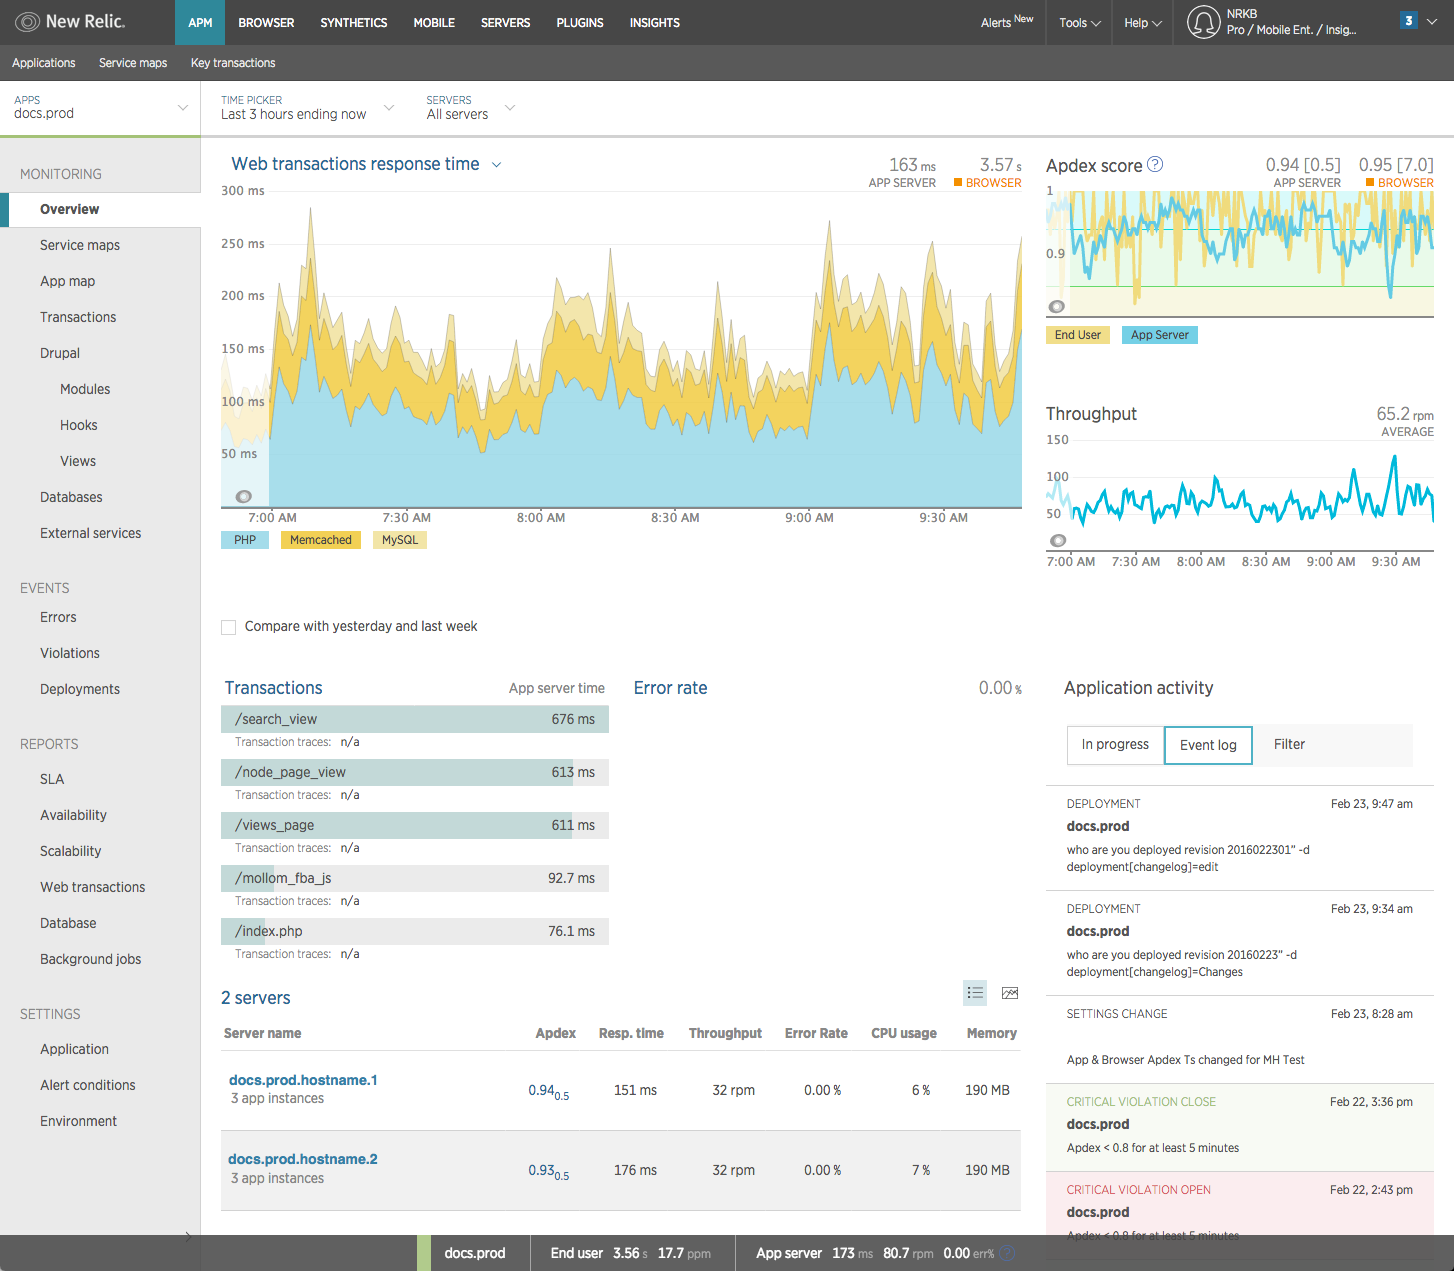
\includegraphics[width=\linewidth]{src/images/anexos/newrelic.png}
  \caption{Cliente web de New Relic}
  \label{fig:new-relic}
\end{figure}

APM es \eng{software} privativo y cuenta con varios planes pagos, según los
requerimientos de los clientes. Dependiendo del nivel de subscripción, es
posible tomar ventaja de diversas prestaciones.

New~Relic tiene una excelente integración con el lenguaje de programación
Ruby~\cite{newrelic}.

\subsection{Google Analytics}

Google Analytics es una herramienta de analítica \eng{web} que ofrece
información agrupada del tráfico que reciben los sitios \eng{web}, según
factores como características de la audiencia, el comportamiento de los usuarios
y las conversiones o hitos alcanzados en el sitio \eng{web}.

Fue creada por Google a partir de un producto anterior comprado por la empresa,
llamado Urchin.

Con Analytics se pueden obtener informes sobre el rendimiento de las páginas,
los resultados de campañas de marketing online, cantidad de sesiones agrupadas
por fuente del tráfico, tasas de rebote, duración de las sesiones y contenidos
visitados, entre otras. \autoref{fig:google-analytics}

\begin{figure}
  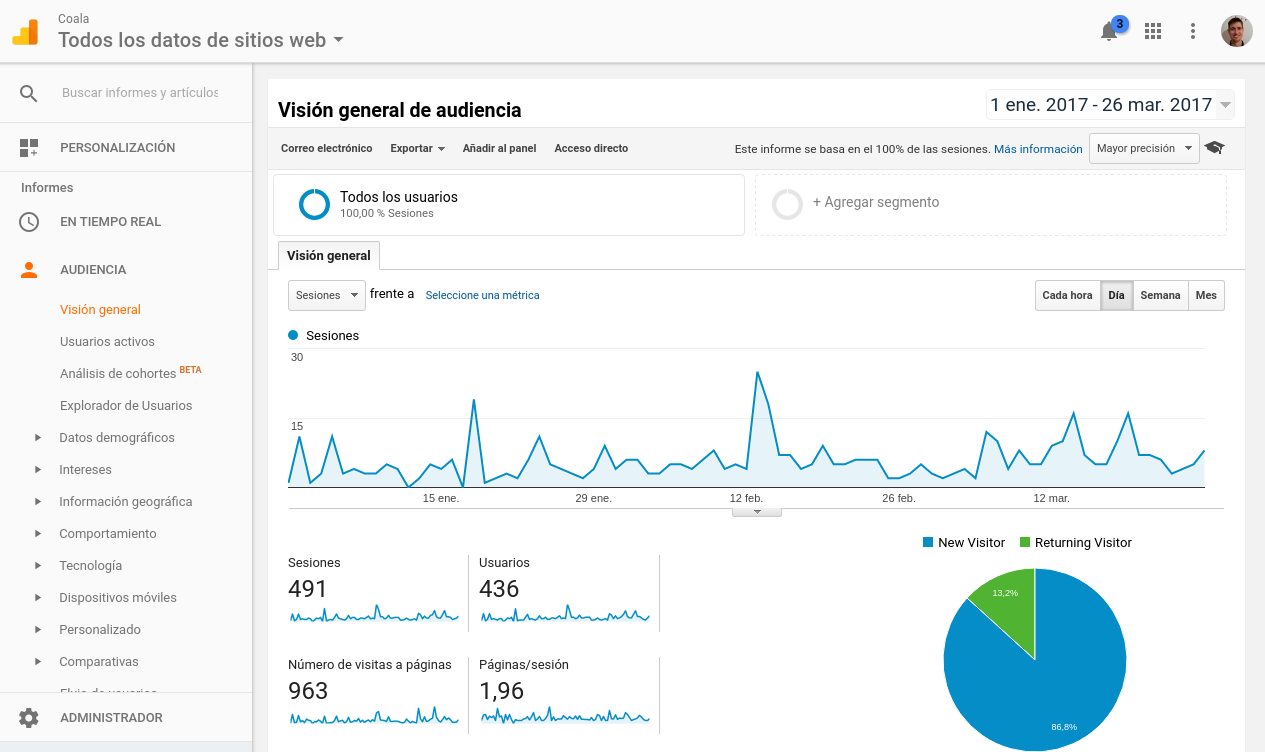
\includegraphics[width=\linewidth]{src/images/anexos/google-analytics.png}
  \caption{Cliente web de Google Analytics}
  \label{fig:google-analytics}
\end{figure}

Para usar esta herramienta en el desarrollo \eng{web}, basta con añadir un
código JavaScript en cada una de las páginas \eng{web} que se desea analizar.

Google Analytics cuenta con una interfaz muy completa de informes con
gráficos~\cite{analytics}.

\subsection{Piwik}

Piwik es un programa completo de \gls{term:php} y \gls{term:mysql} que puede ser
descargado e instalado por los programadores en su servidor \eng{web}. El
proceso de instalación no toma más de 5 minutos. Luego de instalar Piwik se
obtiene un código de Javascript, que se puede copiar y pegar en sitios \eng{web}
de los que se desea hacer un seguimiento y acceder a sus reportes de análisis en
tiempo real.

Piwik dice ser una alternativa de \eng{software} libre a Google Analytics, y al
momento de escribir esta tesis es usado por más de 1.000.000 de sitios
\eng{web}.

Piwik provee reportes de analiticas \eng{web} en tiempo real. Para sitios
\eng{web} de mucho tráfico, es posible elegir la frecuencia con la que los
reportes deben ser procesados.

Como Piwik se encuentra instalado en un servidor personal, los datos son
almacenados en una base de datos propia. Esto significa que uno es dueño de sus
propios datos.

Piwik es \eng{software} libre, y puede ser fácilmente configurado para respetar
la privacidad de los visitantes del sitio \eng{web}. Piwik tiene una comunidad
de más de 200.000 usuarios activos.

Piwik es moderno, y tiene una interfaz que lo hace fácil de utilizar. Es
posible personalizar los tableros y los widgets. \autoref{fig:piwik}

\begin{figure}
  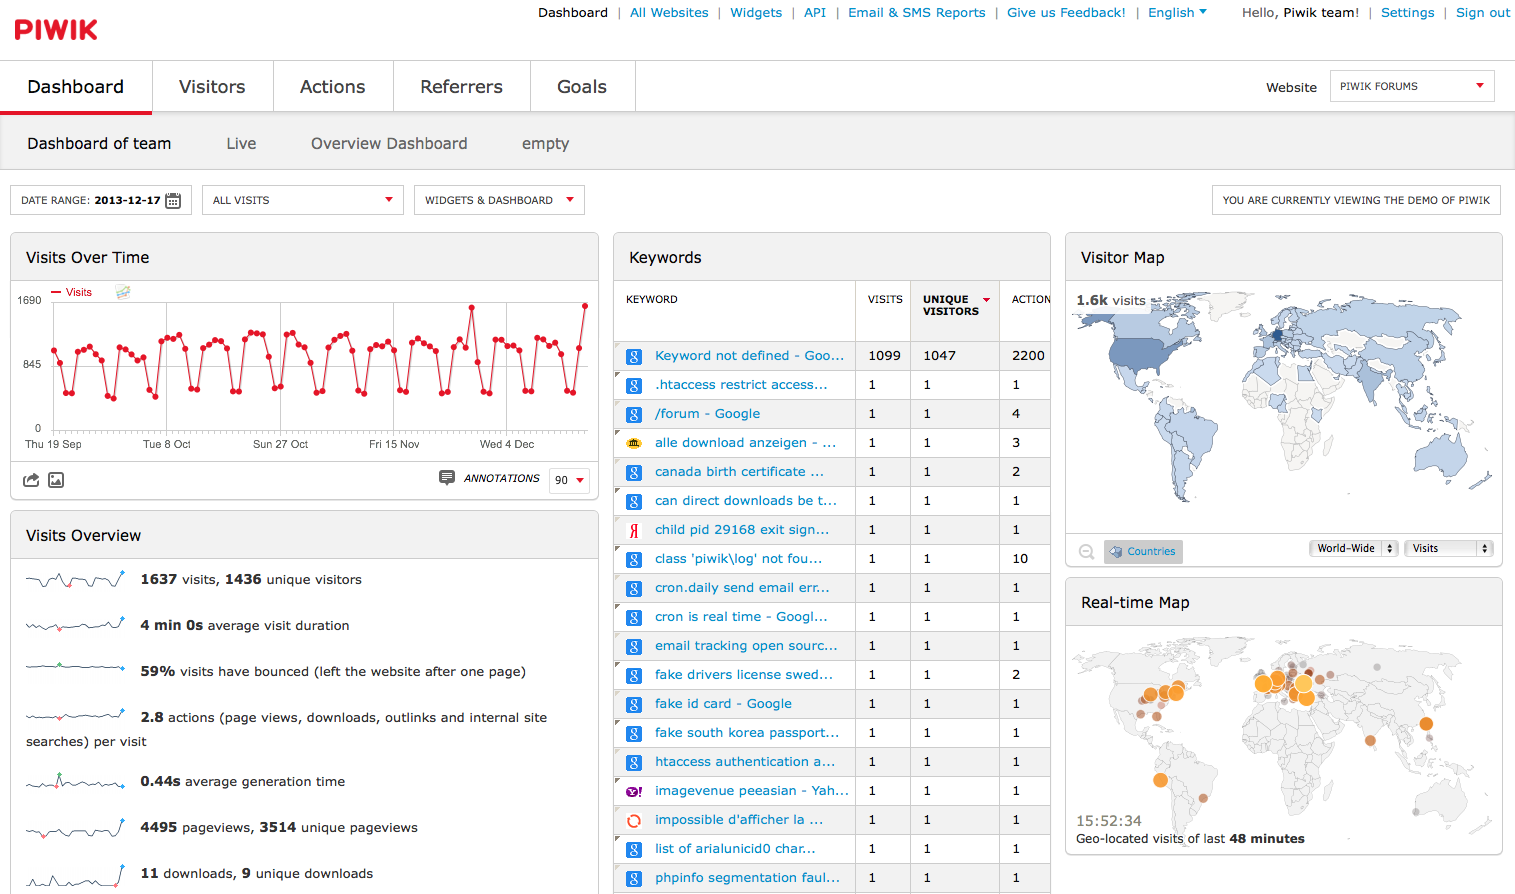
\includegraphics[width=\linewidth]{src/images/anexos/piwik.png}
  \caption{Cliente web de Piwik}
  \label{fig:piwik}
\end{figure}

Piwik tiene avanzadas capacidades de análisis \eng{web}, como seguimiento de
\eng{e-commerce}, seguimiento de metas, seguimiento de campaña, variables
personalizadas, reportes de emails, localización espacial y mapas en tiempo
real~\cite{piwik}.

\subsection{Datadog}

Datadog es un servicio de monitoreo para aplicaciones en la nube, que junta
datos de servidores, bases de datos, herramientas y servicios, y los presenta
en una vista unificada de un \eng{stack} entero. Estas capacidades son provistas
en una plataforma de análisis de datos basada en SaaS (Software como un
servicio).

Datadog usa un agente de código abierto escrito en Python para recolectar
métricas y eventos. Su backend está construido usando un número de tecnologías
de código abierto y cerrado, incluyendo D3, Apache Cassandra, \gls{term:kafka} y
PostgreSQL.

Datadog ayuda a los desarrolladores y equipos de \gls{acro:it} a ver la
infraestructura en un sólo lugar, incluyendo la nube, los servidores, las
aplicaciones, los servicios, las métricas y más.

Datadog incluye tableros interactivos en tiempo real que pueden ser
personalizados para las necesidades específicas de un equipo de trabajo. También
cuenta con la capacidad de realizar búsquedas de texto completo para métricas y eventos, herramientas de colaboración de equipos de trabajo, alertas para problemas críticos y una \gls{term:api} de acceso.

Datadog integra varias herramientas de \eng{software}, de forma que los flujos
de trabajo de equipos no sean modificados ni interrumpidos al adoptar el
servicio de Datadog~\cite{datadog}.

\subsection{Riemann}

Riemann permite la agregación de eventos provenientes de servidores y
aplicaciones utilizando un poderoso lenguaje de procesamiento de
\eng{streaming}.

Puede enviar un email por cada excepción ocurrida en las aplicaciones, mantener
un seguimiento de la distribución de latencia en las aplicaciones \eng{web}, y
observar los procesos principales de cualquier \gls{term:host}, por memoria y
\gls{acro:cpu}.

Puede combinar estadísticas de todos los nodos Riak en un \eng{cluster},
reenviar la información a Graphite, y mantener un seguimiento de la actividad de
los usuarios, segundo a segundo.

Los \eng{streams} de Riemann son simplemente funciones que aceptan un evento.
Los eventos son estructuras con algunos campos comunes, como \gls{term:host} y
service. Es posible usar docenas de \eng{streams} integrados en Riemann para
filtros, alertas y combinación de eventos, y también escribir los propios.

La configuración de Riemann es un programa de Clojure, y por esto su sintaxis
es concisa, regular y extensible. La configuración como código minimiza
repeticiones en código, y otorga la flexibilidad para adaptarse a situaciones
complejas~\cite{riemann}.
